% https://doi.org/10.1364/OE.27.000240
% https://matheo.uliege.be/bitstream/2268.2/6800/6/pvanberg_thesis.pdf    https://ml4physicalsciences.github.io/2019/files/NeurIPS_ML4PS_2019_107.pdf

% https://doi.org/10.1063/1.5125252 <<<<<<

% https://doi.org/10.1038/s41598-020-65417-y

% https://doi.org/10.1364/AO.52.007435

% https://www.vision-systems.com/boards-software/article/14169513/deep-neural-network-accurately-retrieves-phase-information-from-3d-pointspread-functions

% https://doi.org/10.1111/jmi.13083  << Use Z>15

% https://arxiv.org/pdf/2106.04456v1.pdf  << good intro of ML for WF Sensors  || Discussion on fundamental limits.

% https://arxiv.org/pdf/2211.05242.pdf   Zernike distribution, hybrid system

% https://arxiv.org/pdf/1812.01082.pdf

%
% accelerator/ID stuff
% https://doi.org/10.1107/S1600577522008554
% https://journals.aps.org/prab/pdf/10.1103/PhysRevAccelBeams.23.044601


\documentclass[preprint]{iucr}
% \documentclass{iucr}

\usepackage{siunitx}
\usepackage{color}
% \usepackage{amsmath,amssymb}
% \usepackage{amsfonts} 
\usepackage{mathtools}
\usepackage[normalem]{ulem}
\usepackage{adjustbox}
\usepackage{array}
\usepackage{booktabs}
\usepackage{multirow}
\usepackage{alltt}

\newcommand{\todo}[1]{{\color{red}[TODO: "#1'']}}
\newcommand{\remove}[1]{ {\color{blue} \sout{#1}}}
\newcommand{\inblue}[1]{{\color{blue}#1}}
\newcommand{\inred}[1]{{\color{red}#1}}
\newcommand{\ingreen}[1]{{\color{green}#1}}
\newcommand{\soutred}[1]{{\color{red}\sout{#1}}}
\newcommand{\lambdabar}{{\mkern0.75mu\mathchar '26\mkern -8.2mu\lambda}}

\definecolor{JSR_blue}{RGB}{51, 102, 154}
\newcommand{\jsrblue}[1]{\textcolor{JSR_blue}{#1}}

\newcolumntype{R}[2]{%
    >{\adjustbox{angle=#1,lap=\width-(#2)}\bgroup}%
    l%
    <{\egroup}%
}
\newcommand*\rot{\multicolumn{1}{R{90}{1em}}
}


\makeatletter
\@ifclasswith{iucr}{preprint}{
\newcommand{\whencolumns}[2]{#1}
}{
\newcommand{\whencolumns}[2]{#2}
}
\makeatother


 %-------------------------------------------------------------------------
 % Information about journal to which submitted
 %-------------------------------------------------------------------------
 \journalcode{S}

\begin{document}   

\title{X-ray lens figure errors retrieved by deep learning from several beam intensity images}
\shorttitle{MLCRL}

\cauthor[a]{\jsrblue{Manuel}}{\jsrblue{Sanchez del Rio}}{srio@esrf.eu}{}

\author[a]{\jsrblue{Rafael}}{\jsrblue{Celestre}}\aufn{now at: Synchrotron SOLEIL, L'Orme des Merisiers Départementale 128, 91190 Saint-Aubin, France.}
\author[a]{\jsrblue{Juan}}{\jsrblue{Reyes-Herrera}} 

\aff[a]{The European Synchrotron, 71 Avenue des Martyrs, 38000 Grenoble, {France}}

\maketitle                        % DO NOT DELETE THIS LINE

\begin{synopsis}
We demonstrate that a neural network trained with a few thousand simulations using random errors can predict accurately the lens error profile that accounts for all aberrations of a compound refractive lens in a synchrotron beamline. 
\end{synopsis}

\begin{abstract}
We address the phase problem in the context of focusing synchrotron beams with x-ray lenses. We demonstrate the feasibility of retrieving the surface error of a lens system by using only the intensity of the propagated beam at several distances. A neural network, trained with a few thousand simulations using random errors, is able to predict accurately the lens error profile that accounts for all aberrations. It demonstrates the feasibility of routinely measuring the aberrations induced by an x-ray lens, or another optical system, using only a few \inred{intensity} images. 
\end{abstract}


%-------------------------------------------------------------------------
% The main body of the paper
%-------------------------------------------------------------------------


\section{Introduction}\label{sec:intro}

It is well known that the performances of the optical elements in  a synchrotron beamline are limited by surface errors \inred{\cite{Yabashi2014, Schroer2014, Cocco2022}}. The surface errors originate aberrations in the x-ray beam, modifying its properties and limiting the required capabilities (usually focusing, but also affecting collimation and even energy resolution). Moreover, with the advent of a new generation of storage-ring sources (like the EBS-ESRF) and X-ray free electron lasers, the requirements on the optics are more and more demanding, as beam quality (small emittance, beam coherence) dramatically improves. Now, beam degradation originated by any defect (either from fabrication, surface errors or from contamination) is amplified with a coherent source. The optics must accomplish its role preserving the good qualities of the wavefront \cite{Cocco2022}. 

Whenever possible, the surface errors must be minimized during the fabrication process. After fabrication, they are measured by the metrology laboratories that most synchrotron facilities have - \inred{see for example \cite{round_robin1, round_robin2, round_robin3}}. This ex-situ characterization is fundamental for the acceptation of the optics prior to the installation in the beamline, but in many cases are not sufficient to determine the aberrations that will produce in the x-ray beam. This is because the optical elements are dynamic and can move (e.g., bendable mirors) or their configuration change (e.g., transfocators that use a large number of x-ray lenses). Moreover, it is always useful to measure the errors using the same probe (light wavelength) that will be used in operation: x-rays. It is therefore convenient to make in-situ (or \textit{at-wavelength}) beamline measurements for the characterization of optical errors. This is done either using some dedicated wavefront sensors \inred{\cite{Mercere2005, Mikhaylov2020}, x-ray phase-sensitive techniques such as speckle-tracking \cite{berujon_theory_2020, berujon_experiments_2020} or ptychography \cite{Schropp2013}}, which require a dedicated infrastructure and experimental plan, or indirectly from the intensity images of a good quality beam. Examples of indirect measurements are the retrieval of the optical surface using images from a scanned slit \cite{Zhang:ve5019}, or looking at the beam evolution recording images at different positions \inred{like the beam caustics presented in \cite{Celestre:yi5119}}. The indirect measurements of the surface errors are much less accurate than the direct in-situ measurements or characterization from metrology laboratories, but have the advantage that can be obtained in a short time using only instrumentation available at the beamline. They are also limited in spatial resolution (highest spatial frequency), which depends on the quality of the beam used as a probe and the detector point spread function. But the main problem of the indirect measurements is the difficulty to obtain the surface deformation profile (thus the errors) from intensity images, as the aberrations are encoded in the wavefront phase, which is not directly measurable. Phase retrieval, or determination of the phase, requires the use of different techniques and algorithms, and use several intensity images.

We analyze here an optical system to focus a synchrotron beam using x-ray lenses. It is derived from a typical beamline configuration at ESRF, in particular for ID18. This system was the object of previous investigations \cite{multioptics}. We solve the problem of phase retrieval from a collection of images measured at different distances around the focus by using a trained neural network. This work, based on simulations, demonstrates the feasibility of measuring the aberrations originated by the x-ray lenses using only intensity measurements in the neighborhood of the focal position. For that, we train a convolutional neural network (CNN) with synthetic profiles obtained from random variations of some generation polynomials. \inred{The shape of these profiles is compatible to what is generally found for embossed 2D lenses \cite{Roth2017} regardless of their radius or curvature \cite{Celestre2020, Seiboth2020, Dhamgaye2020, Celestre:yi5119}.}
% The shape of these profiles is compatible with the experience learned from direct in-situ experiments \cite{Celestre:yi5119}. 

Machine learning is ubiquitous and used in large facilities, like in tokamaks \cite{Degrave2022-ip}, accelerator control \cite{ML_acc_edelen2020} for synchrotron radiation,  setting insertion device parameters \cite{Sheppard:yi5121}, etc. It is also quite popular for the analysis of the aberrations with wavefront sensors \cite{Nishizaki:19, Mockl2019-sr, Vanberg2019}. 
In particular, the analysis of aberrations with deep learning for 3D microscopy applications \cite{Saha2020} has inspired and guided us in our research.     


% We want to apply to our own problems the ideas, results and codes in \cite{Saha2020}.

% \todo{modify this copied text...}
% The emittance of the storage ring source and the surface errors of the optical surfaces are the most critical parameters that define the upper limit for the brilliance of the X-ray beams.
% The emittance is reduced to roughly the diffraction-limit levels in new (fourth-generation) storage rings of recent design and construction (e.g. \cite{ebs}). A further reduction of the emittance below the diffraction-limit level will not imply a practical gain in brilliance. In parallel, the quality of optics has been dramatically improved to accommodate to the more collimated, brighter, and coherent light without degrading the good qualities of the beam required by the next generation of experimental techniques. The wavefront preservation in X-ray beams implies the use of almost perfect optics or advanced methods for correcting wavefront distortion. This is important for the ultimate performance of the existing Free Electron Lasers and new low-emittance storage rings.  

% A deep understanding of how the imperfections in the optics surface affect the beam quality and limit the beamline performances will require, on one side, sophisticated simulation tools based on algorithms supported by geometric and physical optics. On the other side, these computational methods are useless if there is not a good description of the surface errors. For that, a simplified naive model based on statistical parameters (e.g. RMS slope and height errors) is not sufficient. The measurement of the full profiles and/or maps of the optics is nowadays the only realistic way to assess the quality of the mirror and study the performances by computer simulations, before its physical implementation. This is why most facilities count on a metrology laboratory in charge of the measurement, characterization and analysis of the real mirrors in use or to be used at the facility. Moreover, in-situ measurement techniques (e.g. specke-tracking, ptychography, or other X-ray imaging techniques) allow the measurement of the beam distortion and makes possible to retrieve the profile or map of the optical element. 


%-------------------------------------------------------------------------
%-------------------------------------------------------------------------
\section{Methods}\label{sec:methods}
%-------------------------------------------------------------------------
%-------------------------------------------------------------------------

\subsection{Description of the optical system}\label{sec:descriptionsystem}

The optical configuration studied here consists in a single x-ray lens illuminated by a monochromatic x-ray beam emitted by an undulator in the EBS-ESRF storage ring. It is a simplified part of the future EBSL1 beamline.
The x-ray source is a U18 undulator (period $\lambda_u=\SI{18}{\milli\meter}$) with $N_u=138$ periods placed in the center of a straight section of the EBS storage-ring\footnote{We used the electron beam sizes and divergences $\sigma_x=\SI{29.7}{\micro\meter}$,
$\sigma_{x'}=\SI{4.37}{\micro\radian}$,
$\sigma_y=\SI{5.29}{\micro\meter}$,
$\sigma_{y'}=\SI{1.89}{\micro\radian}$, corresponding to beam emittances:  $\varepsilon_x=\SI{130}{\pico\meter \radian}$,
$\varepsilon_y=\SI{10}{\pico\meter \radian}$, and beta functions
$\beta_x=\SI{6.8}{\meter}$,
$\beta_y=\SI{2.8}{\meter}$.
}. The gap is tuned to have the first harmonic at $E=7$~keV (deflecting parameter $K=1.851$). We consider a Be compound refractive lens (CRL) with parabolic profile and overlapping error profile (described later). The lens is located at a distance $p=\SI{65}{\meter}$ from the source. 
A first CRL implements a single-lens with radius at the appex $R=\SI{50}{\micro\meter}$ ($f=\SI{3.952}{\meter}$ at 7~keV), 
 and the aperture (diameter) is $a=\SI{1500}{\micro\meter}$. A second CRL tested uses 10 lenses of the same radius and aperture, therefore with focal distance 10 times shorter.
 Observation screens are placed in the vicinity of the geometrical focus, at an approximated distance $f$ downstream from the lens. 

\subsection{One-dimensional wavefront model of the system}\label{sec:descriptionsystem}
The complexity of modelling accurately and realistically a synchrotron system resides in the fact that the beam is partially coherent. Completely incoherent beams can be simulated using ray tracing, and fully coherent beams with wavefront propagation. Partial coherence use wavefront simulations, but considering multiple wavefronts. Two methods are used: multielectron Monte Carlo simulation \cite{codeSRW_ME} and coherent mode decomposition \cite{Glass2017}. We recently discussed the interest of studying the system in one dimension, and demonstrated the possibility of performing coherent-mode decomposition \cite{multioptics}  using fewer computer resources. We decided to first use this 1D method to study the system in the vertical direction. 
% The beam at the slit plane has a full-width at half-maximum\footnote{This value is for the first mode only. Multimode gives \SI{565}{\micro\meter}} (FWHM) $a_\text{FWHM}=~\SI{362}{\micro\meter}$.
The intensity distribution of the refracted beam recorded at $N_P$ different propagation positions (downstream from the lens) in an interval around the focal length $f\pm\Delta d$, which for the single-lens CRL is \SI{3.592}{\meter}$\pm$\SI{0.5}{\meter}, and for the multi-lens CRL is \SI{0.359}{\meter}$\pm$\SI{0.05}{\meter}.
The CRL is simulated applying the the thin element approximation [\cite{Celestre2020, multioptics}], using the cumulated profile of the CRL (adding one or 10 parabolic profiles, for the single-lens CRL and the multi-lens CRL, respectively) plus the error profile (that considers the cumulated error of all lens interfaces).
The Oasys \cite{codeOASYS} simulation workflow is shown in Fig.~\ref{fig:oasys}. 

\begin{figure}\label{fig:oasys}
    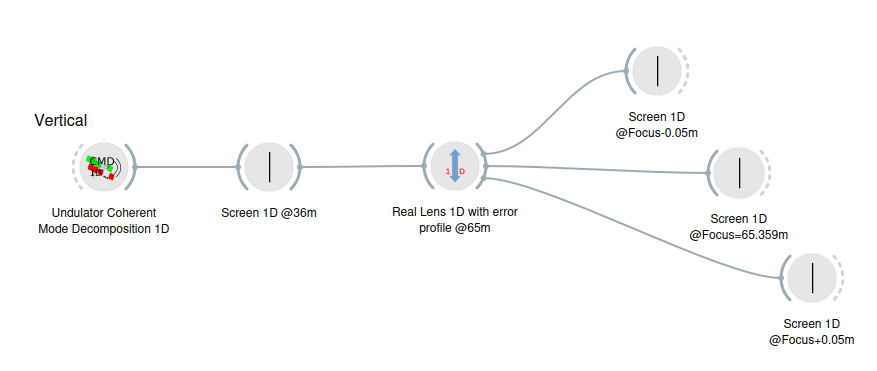
\includegraphics[width=0.99\textwidth]{figures/oasys.png}
    \caption{OASYS workspace containing a flowchart with a single beamline simulation. 
    % \todo{simplify as there are many screens/slits that are not used}
    }
\end{figure}

\subsubsection{Sampling error profiles}
In a simulation, a thin layer of the lens material (Be) with a given profile is added to the parabolic profile of the lens. Lens refraction is simulated using the thin object approximation [see, e.g. \cite{Celestre2020, multioptics}]. Our main objective is to retrieve this profile from the refracted beam intensities. \inred{In the thin element approximation, the error profile in projection approximation $\Delta_z$ is directly proportional to the phase $\phi$ it impinges on the wavefront: $\phi = - \frac{2\pi}{\lambda} \delta \Delta_z$, where $\lambda$ is the wavelength and $\delta$ is the index of refraction decrement as in $n=1-\delta$. Hence, obtaining the error profile from intensity measurements can be seen as a way of addressing the phase problem \cite{Taylor1981,Klibanov1995}.}

To do that, we will train a CNN, but for that, we need a large collection of lens error profiles. We describe here how to parametrize and sample the error profiles to have realistic sampled data. In terms of machine learning [see, e.g. \cite{chollet_book}], this is part of the feature engineering, a process of using your own knowledge about the data and the CNN to make the algorithm work better by applying hardcoded (non-learned) transformations to the data before it goes into the model.
Our experience measuring and analyzing 2D lens profiles indicated that although their topography looks complex, but they can be fitted with great accuracy using the Zernike polynomials \inred{- see comparisons in Figs. 5 to 8 in \cite{Celestre2020}}. In practical terms, it allows expressing our 2D mesh data by only a few Zernike coefficients applied to the polynomial basis (the Zernike polynomials). There are other benefits when using Zernike polynomials: they have some physical meaning, as most of them are associated with a usual aberration (e.g. spherical aberration, coma, etc); and they are orthonormal, thus facilitating the expansion of any profile by just projecting onto the bases \inred{\cite{Mahajan2011}}. In this expansion, the coefficients are non-correlated. Zernike coefficients are often used in deep learning experiments in optics to parametrize the aberrations, typically for wavefront sensing [e.g. \cite{Saha2020}] or in the alignment of the optics [e.g. with Kirkpatrick-Baez mirrors in \cite{Luiz2022}]. 

Error profile samples are by created defining a set of Zernike coefficients with random values. In our case, using Noll notation \cite{Noll:76}, we consider the first 15 polynomials excluding the four first ones (piston, tip, tip and defocus) but adding the secondary and \inred{tertiary} spherical aberrations (Noll numbers 22 and 37). In our case, for 1D simulations in the vertical plane, we are not interested in those with azimuthal dependency, thus ending with 7 polynomials\footnote{in fact, polynomial 12 has been removed as it looks to be easily represented by the others (in the Gram-Schmidt process this was reproduced with a lot of noise). } [6, 8, 10, 11, 14, 22, 37] - \inred{these include astigmatism, trefoil, coma, quadrafoil and primary spherical aberrations}. For each one, a random coefficient should be created. Instead of applying uniform sampling for all of them in the same interval [as done in \cite{Saha2020}], we prefer to customize the ranges and distributions for using empirical experience. We thus sample coefficients using the distributions [n, n, n, u, n, u, u]  (n=normal, u=uniform) and intervals [$\sigma$=0.5, $\sigma$=0.5, $\sigma$=0.5, $\pm$2.3, $\sigma$=0.05, $\pm$1.0, $\pm$0.5] $\times F$ microns, with a factor $F=5$. We sampled $N_P$ 2D mesh surfaces and write the vertical profile in a file, to be used in our wavefront simulations.

The Zernike coefficients are orthonormal on a domain that is a disk of radius unity. If we limit the domain to another shape (e.g. rectangle), or, in our case, we reduce the dimensionality (1D vertical cuts), the Zernike polynomials do not anymore constitute an orthonormal set of polynomials. To solve this inconvenience, with the aim of injecting into the CNN consistent input, we orthogonalized our base of 1D cuts of Zernike polynomials using the Gram-Schmidt method, to obtain a new orthonormal 1D basis. Therefore, the coefficients to be passed to the CNN are those of Gram-Schmidt base, and not those of the 1D Zernike cuts. This does not change the sampled error profiles used in the wavefront simulations, but changes the target values uses to train and test the CNN.  

\subsection{Deep learning system}

Once prepared a collection of $N_S$ sampled profiles, the wavefront simulation is run for each one. For each sample,  we calculate intensity distribution at the $N_P$ propagation images. Each simulated intensity plot has 1500 points. To save data volume, we reduced the number of points by interpolation to $N_A=256$ points (making sure we do not miss characteristic features, structures or artifacts in the intensity distribution). Therefore, the $N_S$ runs of the wavefront simulator produce a stack of $N_S \times N_P \times N_A$ float number values, that constitute the data for the CNN. The target data is a stack of $N_S \times 7$ values, containing the Gram-Schmidt coefficients. The data stack is saved in an \texttt{hdf5} file and the target data in a \texttt{txt} file to be passed to the CNN. Running the wavefront simulations for $N_S=5000$ lasted about 2h in a CPU using a single coherent mode. For partial coherence simulations we propagated 10 coherent modes that contain more than 99\% of the total intensity, therefore it takes about 10 times more running time. Figure~\ref{fig:sample} shows an example of how the data looks for the first sample (defined with no deformation) and for another run.


\begin{figure}\label{fig:sample}
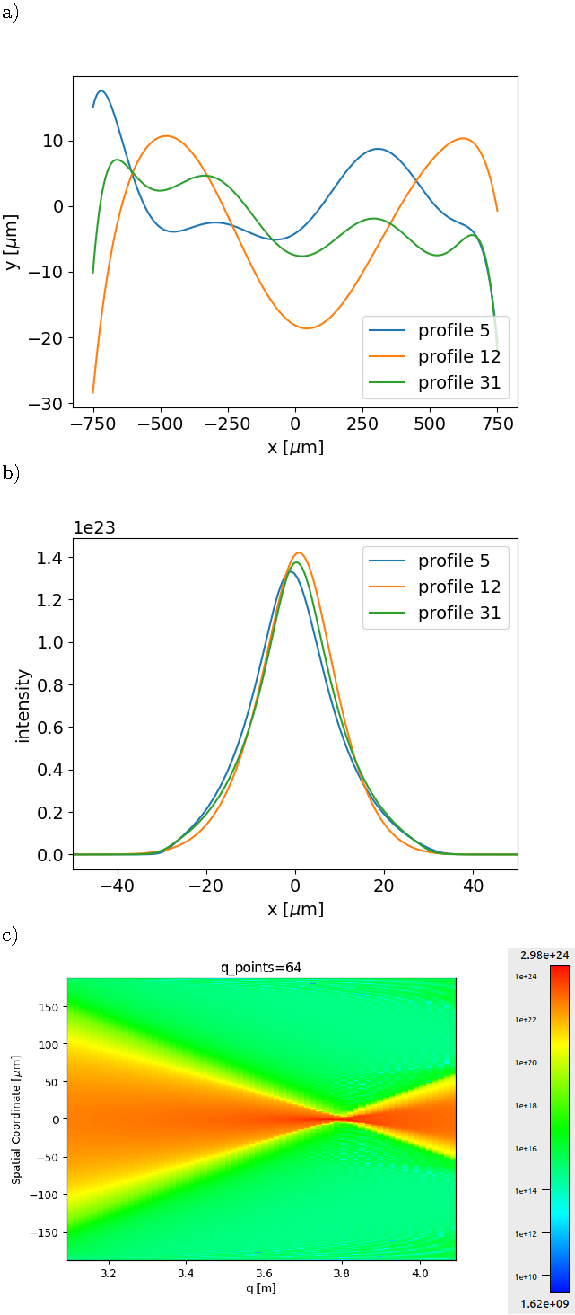
\includegraphics[width=0.55\textwidth]{figures/figure2.pdf}

    % a)~~~~~~~~~~~~~~~~~~~~~~~~~~~~~~~~~~~~~~~~\\ 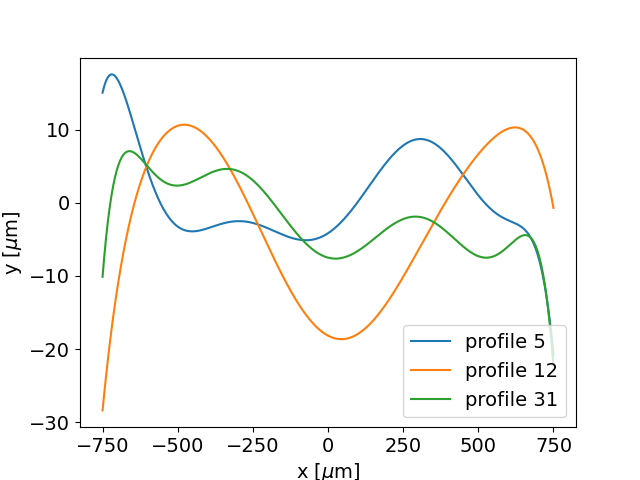
\includegraphics[width=0.8\textwidth]{figures/Figure2a.png}
    % b)~~~~~~~~~~~~~~~~~~~~~~~~~~~~~~~~~~~~~~~~\\ 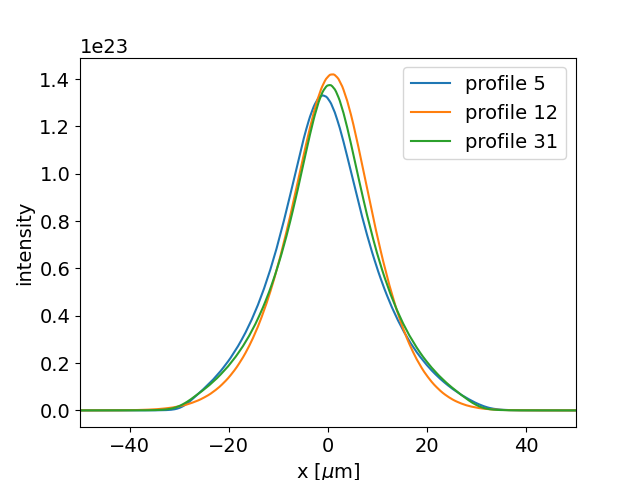
\includegraphics[width=0.8\textwidth]{figures/Figure2b.png}
    % c)~~~~~~~~~~~~~~~~~~~~~~~~~~~~~~~~~~~~~~~~\\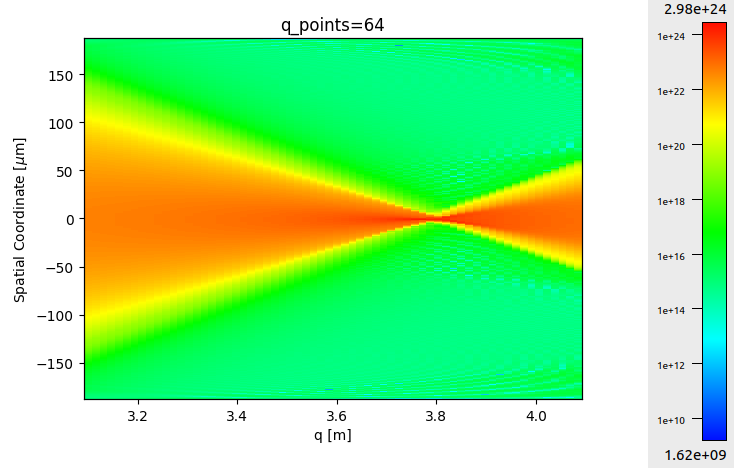
\includegraphics[width=0.8\textwidth]{figures/Figure2c.png}
    
    \caption{Examples or lens error profiles and intensity profiles. a) Three error profiles, b) their corresponding intensities at the center of the propagation interval, and c) propagation or caustic plot in the full interval for error profile number 5 (color in log scale). The CRL is made of a single lens, and only the first coherence mode is used.
    }
\end{figure}

We created a CNN using Keras \cite{keras} with architecture similar to PHASENET \cite{Saha2020}. It consists of five stacked blocks, each comprising two $(3 \times 3 )$ convolutional layers (with stride 1 and the number of channels doubling every block starting with 8) and one max-pooling layer (only along the lateral dimensions), followed by two dense layers (64 channels) and a final dense layer having the same number of neurons as the number of Gram-Schmidt coefficients to be predicted (7 in our case). We use \texttt{relu} as activation function for all layers except the last, where we use linear activation. This results in a rather compact CNN model with a total of 430655 parameters.

To prevent overfitting, we look at the accuracy of the training and validation data (a 20\% fraction) and verified a uniform parallel increasing accuracy on the training and validation sets. If needed, we rerun the training with increased $N_S$. The possibility to increase more and more $N_S$ (i.e. having an ilimited number of samples) is the great advantage of using synthetic data for training the CNN, and makes not necessary the use of regularization techniques to avoid overfitting.

We minimize the mean squared error (MSE) between predicted and ground truth coefficients and train each model for $N_E$ epochs and batch size 64 on a GPU (NVIDIA Tesla V100-SXM2-32GB) using the RMSprop optimizer with learning rate 10$^{-4}$ for a total training time of less than one hour.


%-------------------------------------------------------------------------
%-------------------------------------------------------------------------
\section{Results for the 1D propagation model}\label{sec:results}

The design and optimization of a deep learning system is more an art than a science \cite{chollet_book} and the experience is a real asset. We describe here our procedure, which follows the experience found in the literature. As discussed before, we started with a model similar to PHASENET \cite{Saha2020} which some differences to fit our needs: 
\begin{enumerate}
    \item We use a 1D propagation model, therefore our input data has dimension $(N_P,N_A)=(64,256)$ instead of (32,32,32). We then use \texttt{Conv2D} instead of \texttt{Conv3D} layers. 
    \item Our simulation process bases on wavefront propagation is more complex and CPU-demanding, therefore it has been uncoupled from the training. Therefore, we run first the simulations in a CPU, and then the training in a GPU.
    \item We use \texttt{relu} instead of \texttt{tanh} activation (a preliminary run showed much better convergence). 
\end{enumerate}

 We use 2/3$\times N_S$ samples for training (80\% for true training and 20\% for validation) and 1/3$\times N_S$ for testing. 
 
 \subsection{Results for CRL made of a single lens}
 The accuracy of the training and validation data is shown in Fig~\ref{fig:v12v13} versus the number of epochs.
 We made the first run with $N_S=1000$.
 It is remarked (Fig~\ref{fig:v12v13}a) how the learning slope reduces at about 300 epochs. The accuracy of the test data is 79\%.
 % The predictions for the test data, although matching the general trend, are not satisfactory from the quantitative point of view (Fig~\ref{fig:v12v13profiles}a). 
 Clearly, more samples are needed. We then run $N_S=5000$ samples. The accuracy of the test data improved to 93\% (Fig.\ref{fig:v12v13}b).
 % and the predicted profiles for the test data are very close to the original ones (Fig.\ref{fig:v12v13profiles}b). 
 We consider that this CNN model works satisfactorily and label it as our standard configuration. Further tests will follow to study how some changes in the configuration and parameters may influence the results.

\begin{figure}\label{fig:v12v13}
    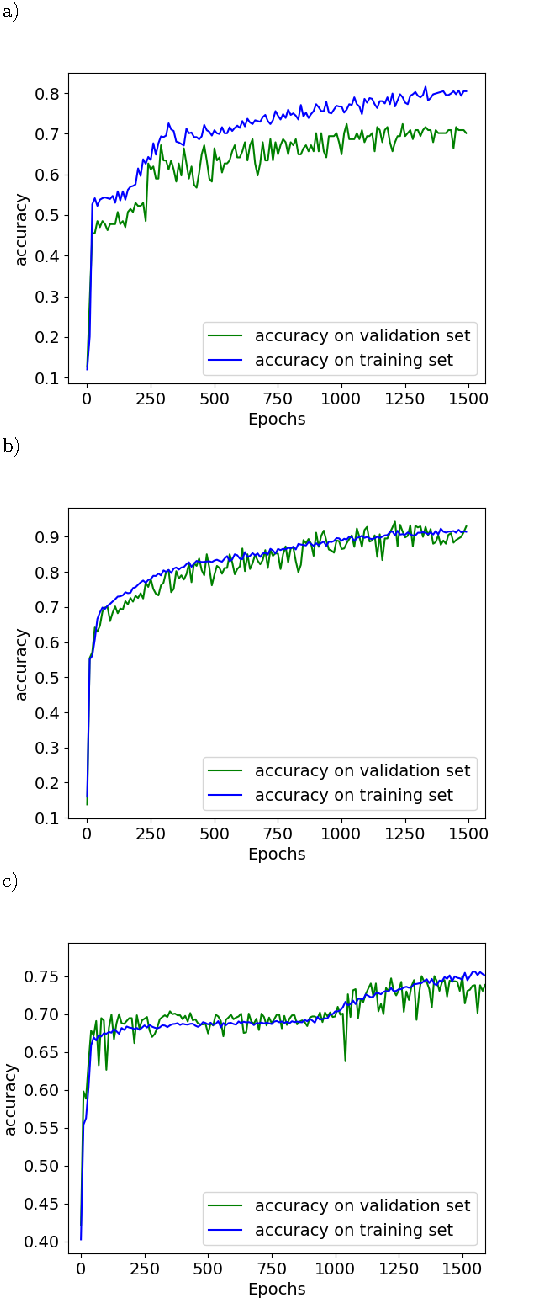
\includegraphics[width=0.55\textwidth]{figures/figure3.pdf}
    % a)~~~~~~~~~~~~~~~~~~~~~~~~~~~~~~~~~~~~~~~~~~~~~~~~~~~~~~~~~~~\\    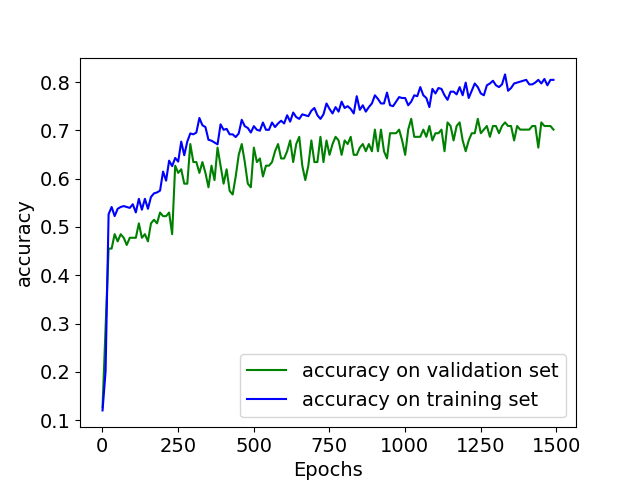
\includegraphics[width=0.75\textwidth]{figures/v12.png}
    % b)~~~~~~~~~~~~~~~~~~~~~~~~~~~~~~~~~~~~~~~~~~~~~~~~~~~~~~~~~~~\\ 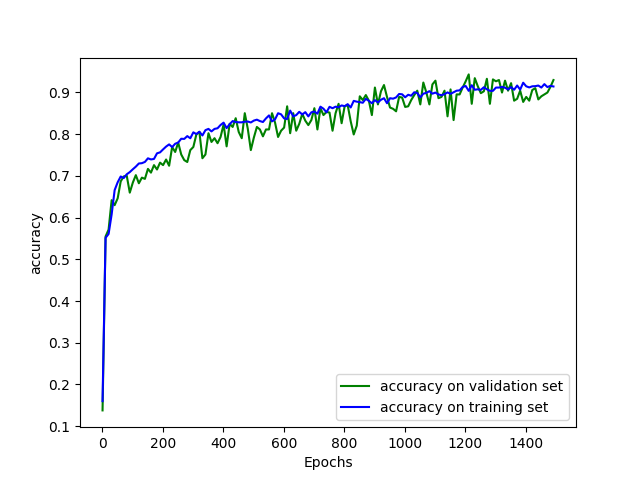
\includegraphics[width=0.75\textwidth]{figures/v13.png}
    % c)~~~~~~~~~~~~~~~~~~~~~~~~~~~~~~~~~~~~~~~~~~~~~~~~~~~~~~~~~~~\\ 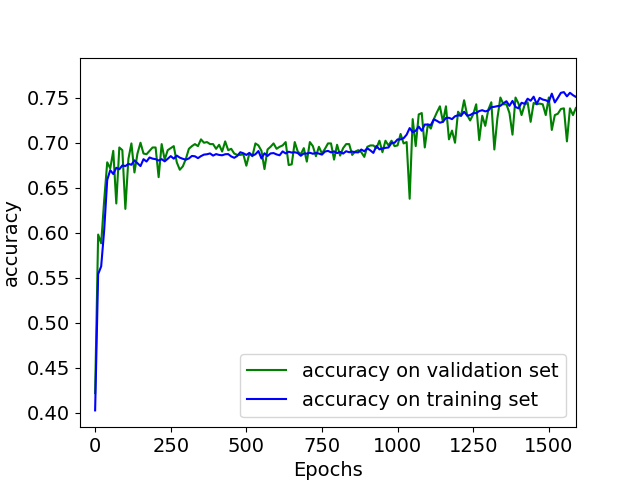
\includegraphics[width=0.75\textwidth]{figures/v25.png}
    \caption{Accuracy of the training data and validation data, for a) single-lens CRL $N_S$=1000, b) single-lens CRL $N_S$=5000, and c) multi-lens CRL $N_S$=10000.
    }
\end{figure}



% \begin{figure}\label{fig:v12v13profiles}
%     a)~~~~~~~~~~~~~~~~~~~~~~~~~~~~~~~~~~~~~~~~~b)~~~~~~~~~~~~~~~~~~\\
%     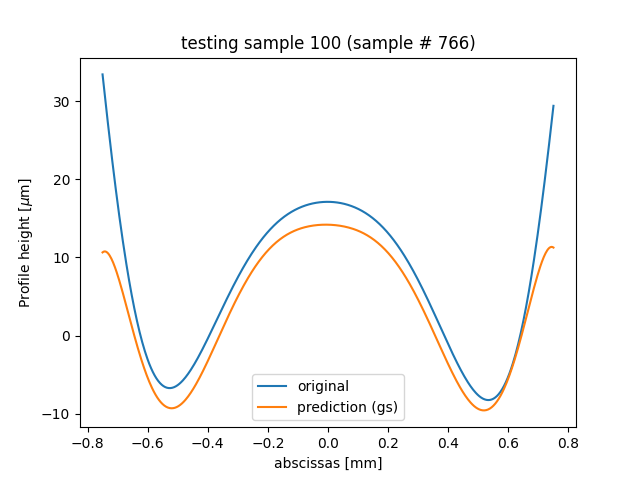
\includegraphics[width=0.45\textwidth]{figures/v12p100.png}
%     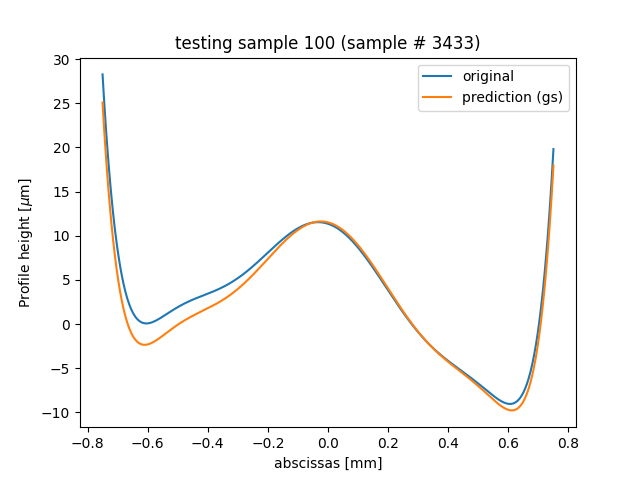
\includegraphics[width=0.45\textwidth]{figures/v13p100.png}

%     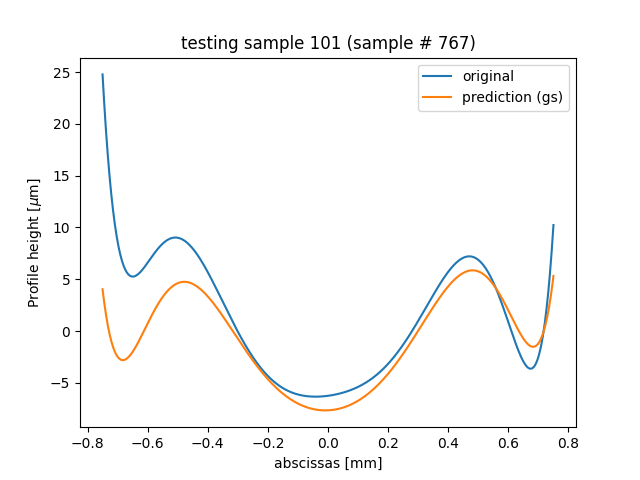
\includegraphics[width=0.45\textwidth]{figures/v12p101.png}
%     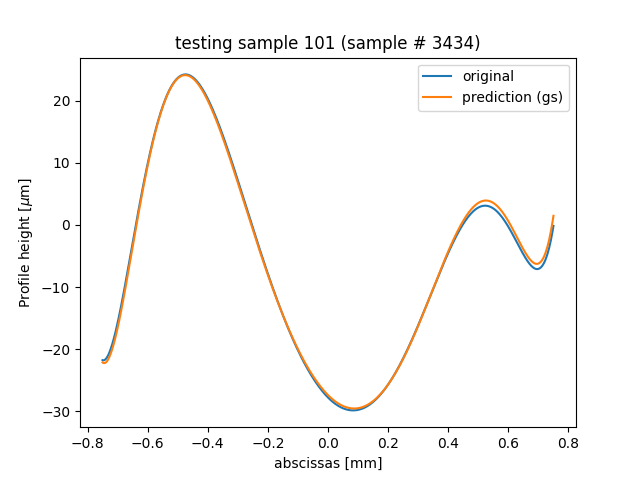
\includegraphics[width=0.45\textwidth]{figures/v13p101.png}

 
%     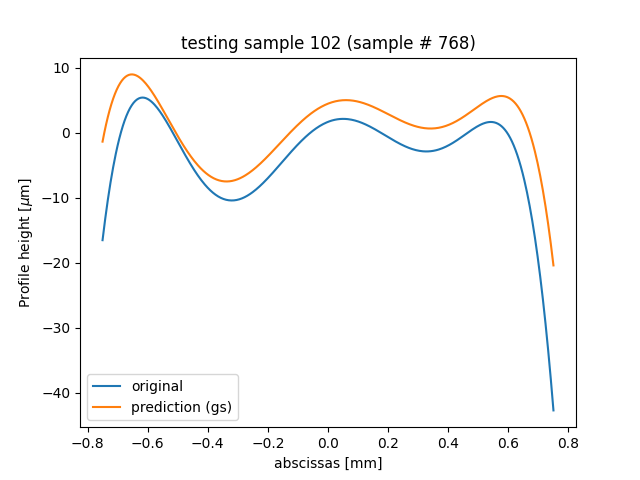
\includegraphics[width=0.45\textwidth]{figures/v12p102.png}
%     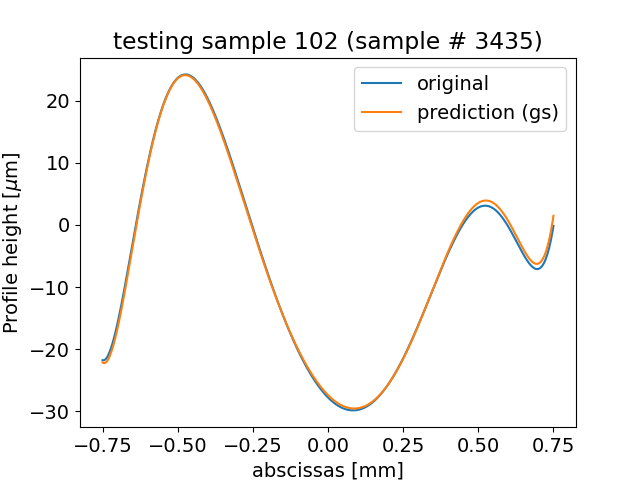
\includegraphics[width=0.45\textwidth]{figures/v13p102.png}

    
%     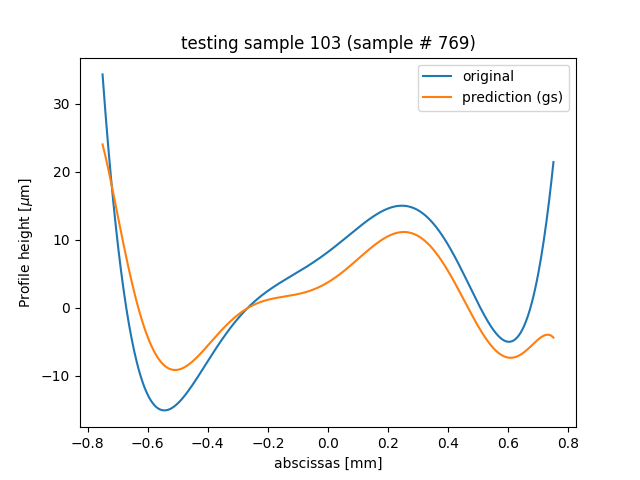
\includegraphics[width=0.45\textwidth]{figures/v12p103.png}
%     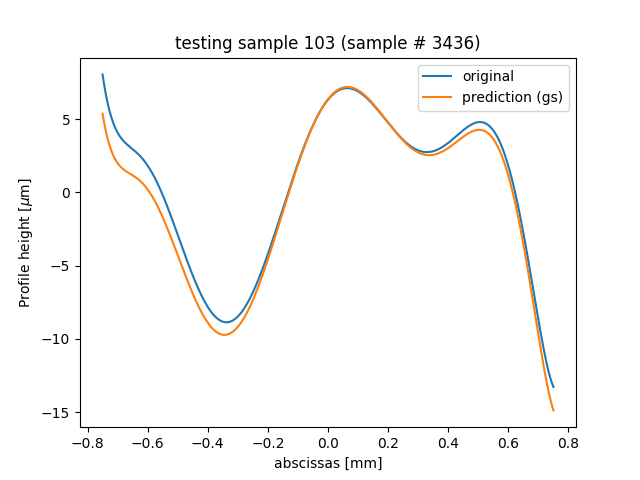
\includegraphics[width=0.45\textwidth]{figures/v13p103.png}

%     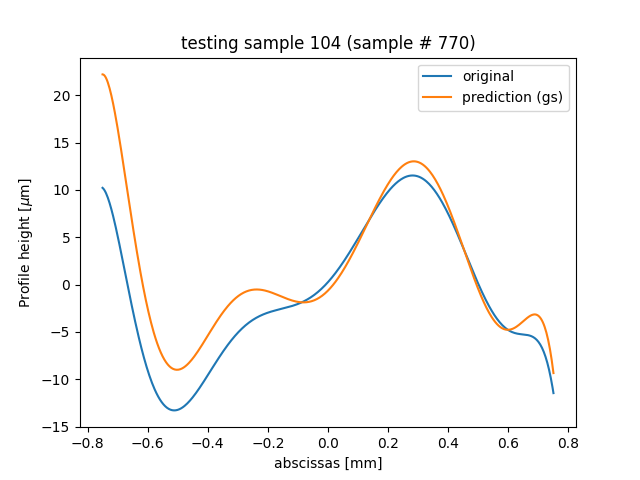
\includegraphics[width=0.45\textwidth]{figures/v12p104.png}
%     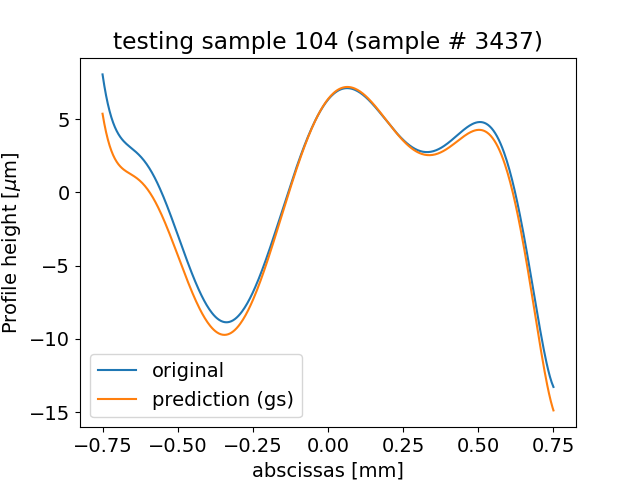
\includegraphics[width=0.45\textwidth]{figures/v13p104.png}


%     \caption{Some original and fitted (predicted) profiles from samples in the test data. a) (left column): $N_S$=1000 (accuracy on test data 79\%), b) (right column): $N_S$=5000 (accuracy on test  data 93\%). 
%     % Right column: $N_S$=5000 using Zernike (instead of Gram-Schmidt) coefficients (accuracy on test  data 91\%). \todo{overplot the Zernike coefficients} \inred{(I overplotted in green the points used in wofry to be sure there is no error in picking the data)}
%     }
% \end{figure}

 \subsection{Results for a CRL made of 10 lenses}
 This case implements 10 lenses, with a shorter $f$. The accuracy of the training and validation data is shown in 
 Fig~\ref{fig:v12v13}c.
 It can be noticed a much worse accuracy (0.73) as compared with the case of a single lens (0.93). The number of samples has been raised to $N_s$=10000. The reason of the worse training is due to the higher absorption of the CRL in the multi-lens CRL case: the cumulated absorption over the 10 lenses reduces significantly the tails of the intensity distribution to almost zero, thus the system does not respond to changes in the error profile in this zone. This will be further discussed in the next section.



\section{Discussion}\label{sec:discussion}

We analyze here the influence of several parameters, concerning the learning procedure and also the influence of some physical aspects, like the use of a partially coherent beam.

% A first question is whether we improve the learning (getting a better accuracy value) by incrementing the number of epochs. Our tests showed that incrementing the number of epochs does not improve significantly the accuracy. The overfitting point (where the accuracy on the training and on the validation data crosses) is about the number of epochs used. To effectively improve the learning we would need more samples. \inred{for the CRL made of a single lens the overfitting point is around 1500 epochs. For the CRL with 10 lenses, it is XXXX.}


\subsection{Use of orthornormal basis.} The question is whether the use of an orthonormal basis for expressing the target coefficients is important. We tested the system using as targets in the training procedure the Zernike 1D coefficients instead of the Gram-Schmidt ones. As expected, the results are not so good: although 
accuracy is only two points below (91\% instead of 93\%), the predicted profiles agree visually less well to the true profiles is worse (Fig.~\ref{fig:v14profiles}). However, a system using decomposition in non-orthogonal coefficients also well. 


\begin{figure}\label{fig:v14profiles}
    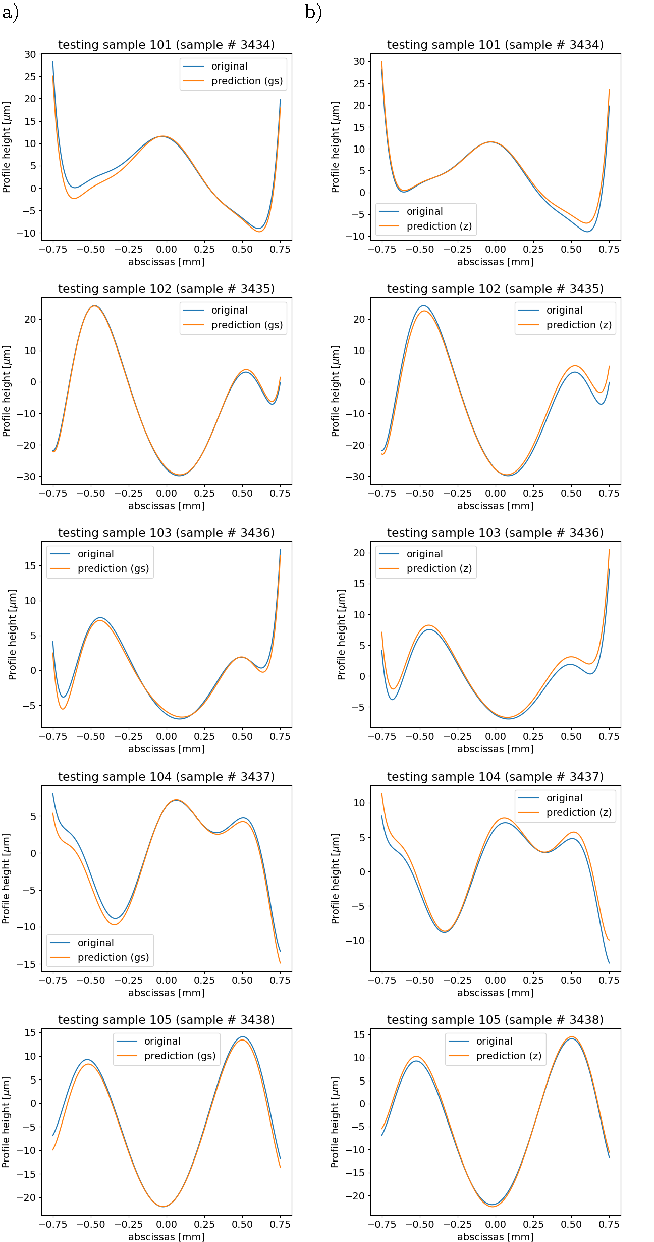
\includegraphics[width=0.75\textwidth]{figures/figure4.pdf}
    % a)~~~~~~~~~~~~~~~~~~~~~~~~~~~~~~~~~~~~~~~~~b)~~~~~~~~~~~~~~~~~~\\
    % 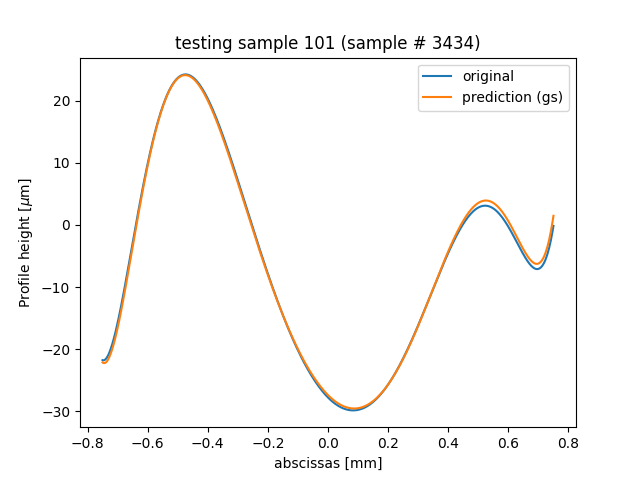
\includegraphics[width=0.45\textwidth]{figures/v13p101.png}
    % 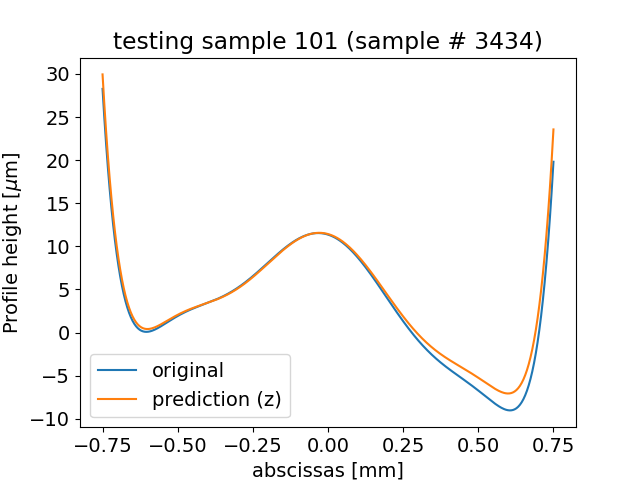
\includegraphics[width=0.45\textwidth]{figures/v14p101.png}

    % 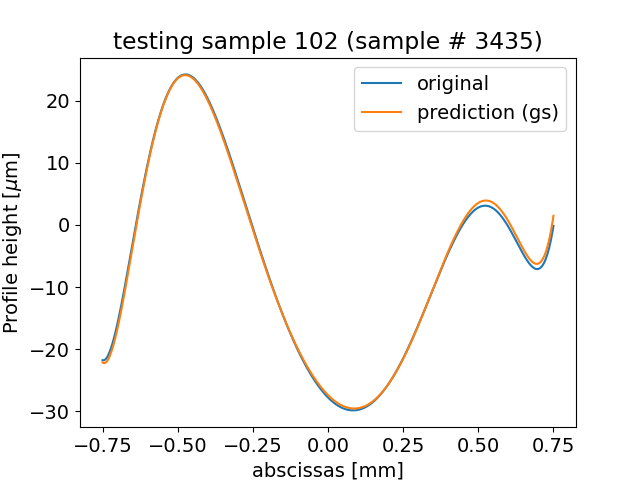
\includegraphics[width=0.45\textwidth]{figures/v13p102.png}
    % 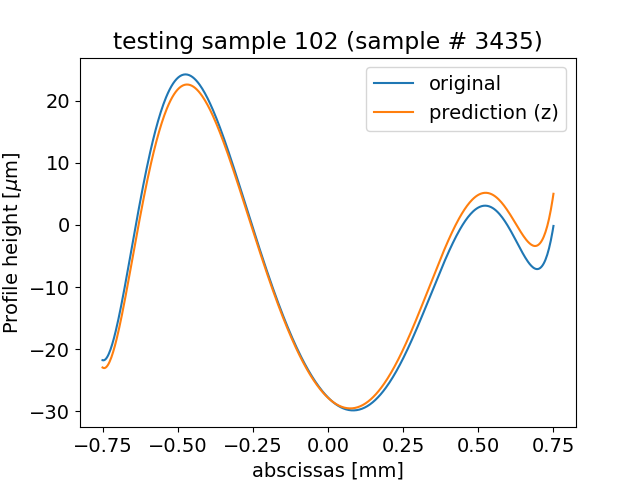
\includegraphics[width=0.45\textwidth]{figures/v14p102.png}

 
    % 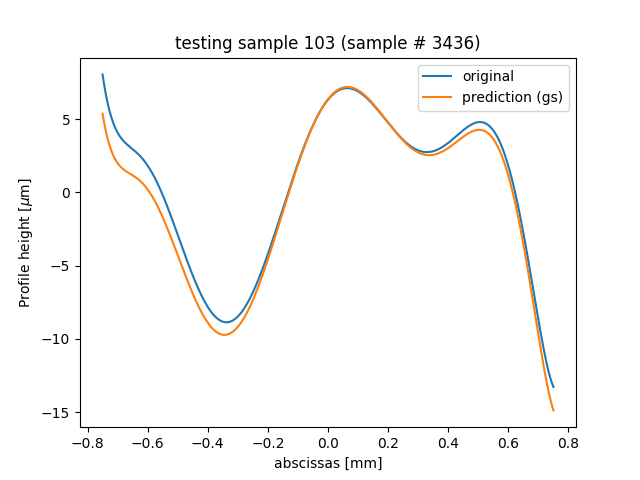
\includegraphics[width=0.45\textwidth]{figures/v13p103.png}
    % 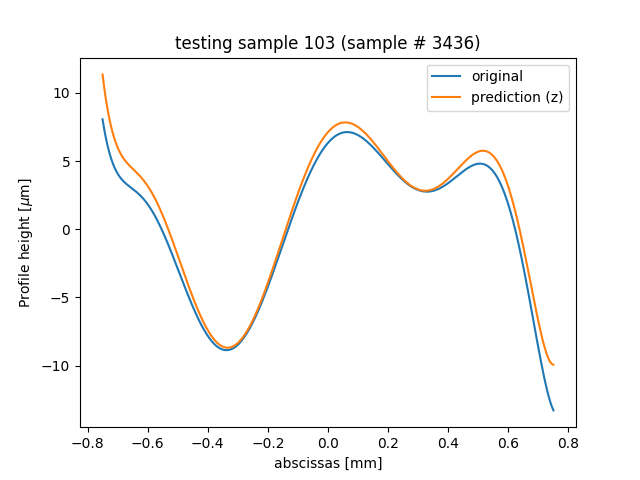
\includegraphics[width=0.45\textwidth]{figures/v14p103.png}

    
    % 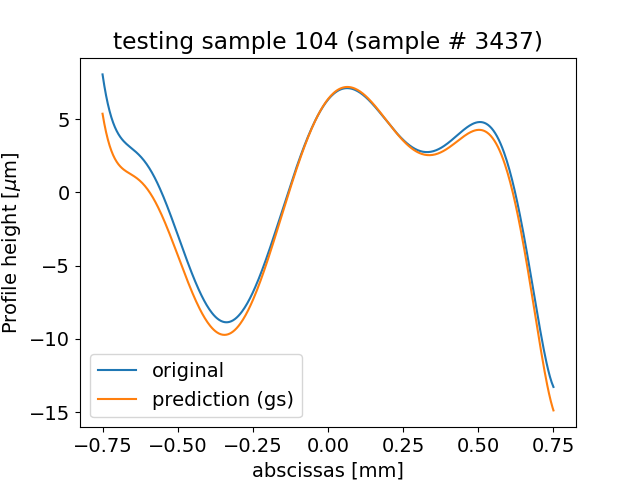
\includegraphics[width=0.45\textwidth]{figures/v13p104.png}
    % 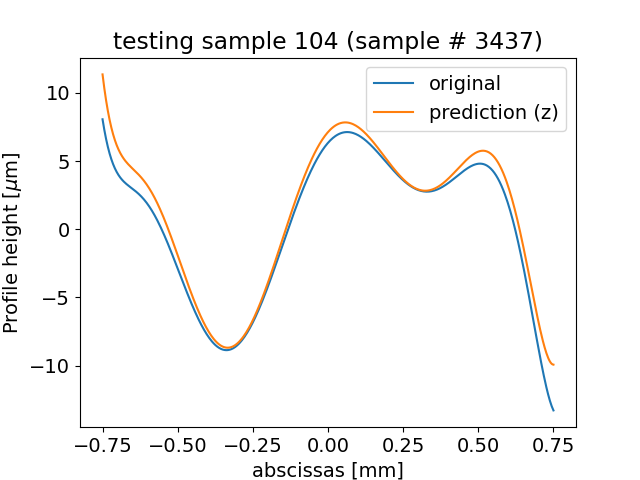
\includegraphics[width=0.45\textwidth]{figures/v14p104.png}

    % 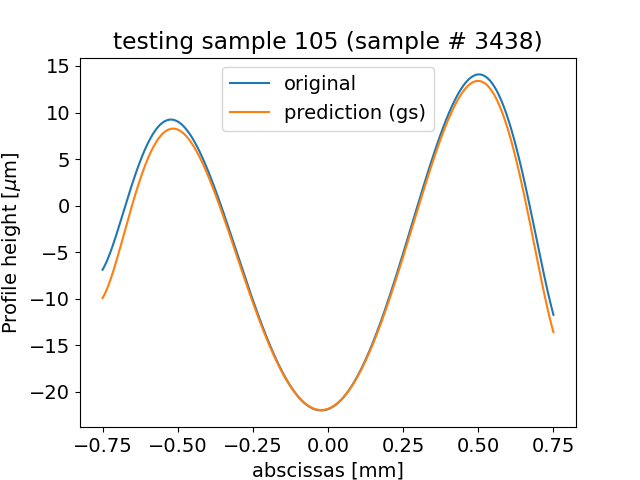
\includegraphics[width=0.45\textwidth]{figures/v13p105.png}
    % 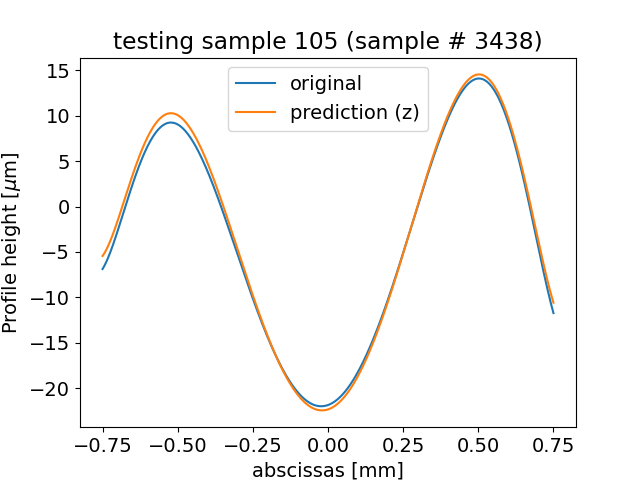
\includegraphics[width=0.45\textwidth]{figures/v14p105.png}

    \caption{Some original and fitted (predicted) profiles from samples in the test data. a) (left column): Standard model $N_S$=5000 (accuracy on test  data 93\%) using Gram-Schmidt bases;
    b) The same model trained with targets using  non-orthogonal 1D Zernike bases (accuracy on test  data 91\%). Note that although the difference in accuracy is only 2\%, there are appreciable differences in the profiles.
    }
\end{figure}


\subsection{Capacity of the CNN.}
We analyzed the possibility to reduce the capacity of the CNN. Our 1D model is much simple than a full 2D model in \cite{Saha2020}, thus each sample requires less data (we have $N_P\times N_A=64\times 256$ float-numbers instead of $32^3$ in PHASENET). The question is whether we can strongly reduce the capacity of the CNN. The answer is yes, but we would need more samples to get the same accuracy as in our standard configuration. If we remove the last convolutional block (which has the highest capacity) we get for the CRL system with a single lens an accuracy value of 86\% (instead of 93\% for the standard configuration).


\subsection{Effect of the number of the image planes and their position.}
Thinking about the possible experimental realization of the system discussed here, it is important to make economies in the number of images to be acquired ($N_P$), and also the scanning interval. Ideally, the highest $N_P$ and the higher interval, the better. But the experimental setup limits the interval, and the recording time limits $N_P$. This is also discussed in \cite{Saha2020} showing that a reduction in the number of images is possible at the price of a less good learning and the minimum number of images is somehow related to the number of target coefficients in use. We trained the CNN with less image planes by just picking the calculated data with frequency 2 ($N_P=32$) and 4 ($N_P=16$), resulting in an accuracy of 84\% and 85\%, respectively (compared with the initial 93\%). 
We also looked at what happens if we scan the image plane out of focus. We used the calculations on the 32 planes downstream from focus, and got good accuracy (92\%) but with a much different learning curve with a step-down at about 700 epochs. Stopping the learning at this point, we obtained an accuracy of 90\%, also showing that the system still works well. 
% (Fig.\ref{fig:v19})]. Stopped at 700 epochs (90\%).

% Try less image planes. What is reasonable? [
%     v15: nbin=2 (32 planes) val\_accuracy=84\%; 
%     v16: nbin=4 (16 planes) val\_accuracy=85\%;
%     ]

% Scan the image plane out of focus. Better or worse?
% [Used 32 planes downstream from focus. 92\% but with a strange curve (Fig.\ref{fig:v19})]. Stopped at 700 epochs (90\%).

\subsection{Partial coherence.}
The quality of the intensity images (the features in our CNN) is extremely important. The presence and detectability of some structures are fundamental to be able to retrieve the target profile. Consequently, a beam with less quality will produce worse images and therefore slow down the CNN learning (thus requiring more cycles or more data). In the limit, if the quality of the beam is too bad, the system simply does not work.  

There are several physical factors that define the quality of the beam. We are affected by the emittance and coherence. In most works related to wavefront sensors, the beam is ``prepared" to record the point spread function. Usually this is achieved using a pinhole that will produce something that approximates a point source. In our case we do need a pinhole or slit, and we can use the direct synchrotron beam due to the low emittance of the 4$^\text{th}$ generation of synchtroton storage rings. The other parameter to look at is the coherence. Synchrotron radiation is not fully coherent, and is less and less coherent when increasing the photon energy. In the case analyzed here, the coherent fraction in the vertical direction of the undulator source at 7 keV is about 0.6 [see \cite{multioptics} for a full discussion], therefore the beam cannot be considered fully coherent. An analysis of the coherence can be done using coherent mode decomposition (ibid). This means that the source is decomposed in a number of coherent modes (wavefronts) that should be propagated one by one and add their individual contributions to the intensity of the image. We re-run the simulation using partial coherence. Ten modes are enough to model with high quality the partially coherent beam (representing more than 99\% of its intensity). Although the volume of data created for the CNN training is the same, the calculation requires more than 10 times more time. The new results are used to train the CNN with the same parameters as the standard model. In Fig.~\ref{fig:multimode}a we can see the learning curves, manifesting a clear underfitting but arriving accuracy of 92\%. Increasing more and more (up to 25000) the number of epochs we see that the system improves (Fig.~\ref{fig:multimode}b). It is about $N_E=1000$ when the accuracy of the training and validation sets cross. However, although the accuracy on the validation set does not increase anymore, it does not decrease, ending in a value of 97\%. Fig.~\ref{fig:multimode} show some of these profiles for comparison.

Therefore, the use of a partially coherent beam (instead of the fully coherent beam) just slows down the learning process but it is not a limiting factor for retrieving the target coefficients with high accuracy. Although it is dangerous to extrapolate this conclusion to different systems, it is very useful to know that simulations with full coherence are good approximations to model the system. Thus, they can be used for creating synthetic training data with a much reduced computational cost. 

 
\begin{figure}\label{fig:multimode}
    a)~~~~~~~~~~~~~~~~~~~~~~~~~~~~~~~~~~~~~~~~~~~~~~~~~~~~~~~~~~~~~~~~~~~~~~~~~~~~~~~\\
    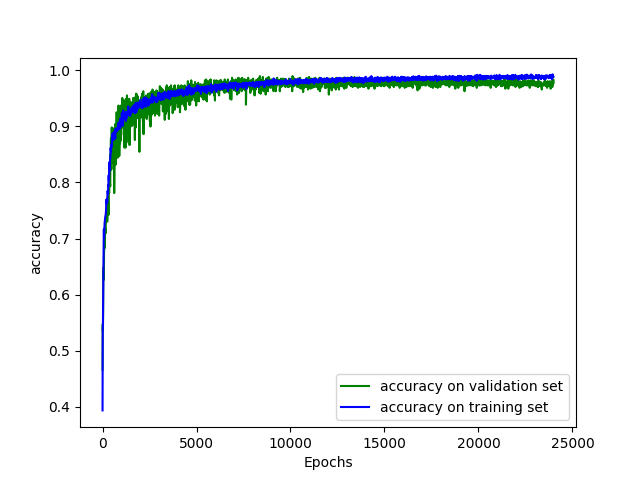
\includegraphics[width=0.8\textwidth]{figures/v23.png}
    
    b)~~~~~~~~~~~~~~~~~~~~~~~~~~~~~~~~~~~~~~~~~~~~~~~~~~~~~~~~~~~~~~~~~~~~~~~~~~~~~~~\\
    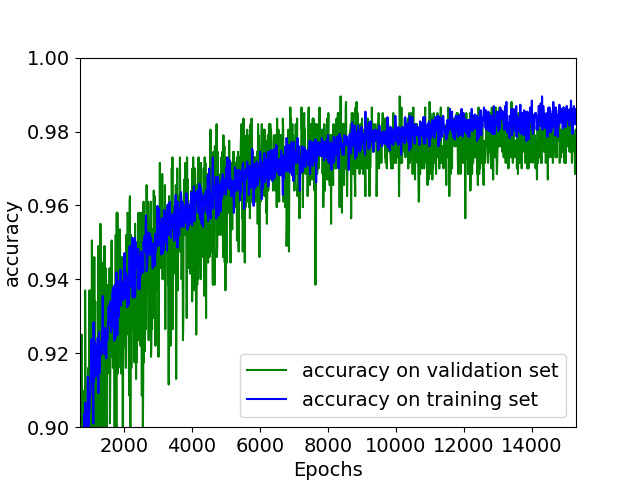
\includegraphics[width=0.8\textwidth]{figures/v23zoom.png}
    % b)~~~~~~~~~~~~~~~~~~~~~~~~~~~~~~~~~~~~~~~~~~~~c)~~~~~~~~~~~~~~~~~~~~~~~~~~~~~~~~~~~~\\
    % 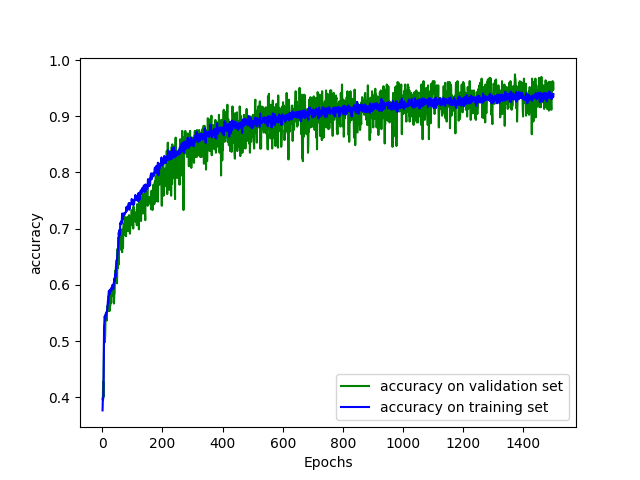
\includegraphics[width=0.49\textwidth]{figures/v20.png}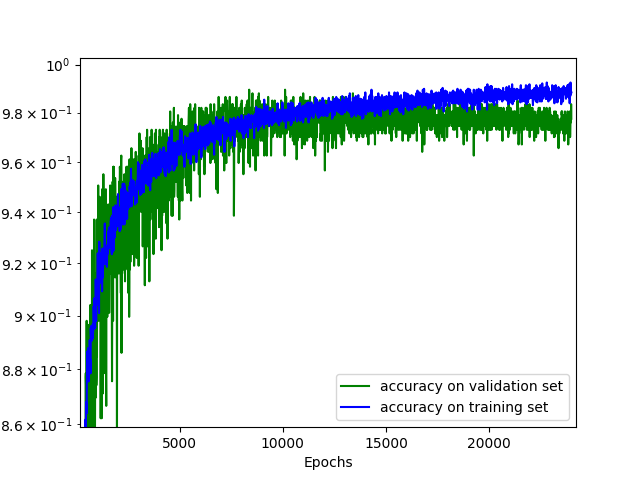
\includegraphics[width=0.49\textwidth]{figures/v23z.png}
    \caption{Accuracy of the training data and validation data, for partial coherence calculations top) $N_S$=5000 64 planes downstream from focus, 25000 epochs;
    b) the same zoomed to observe the crossing point around 10000 epochs.
    }
\end{figure}

\begin{figure}\label{fig:multimode}
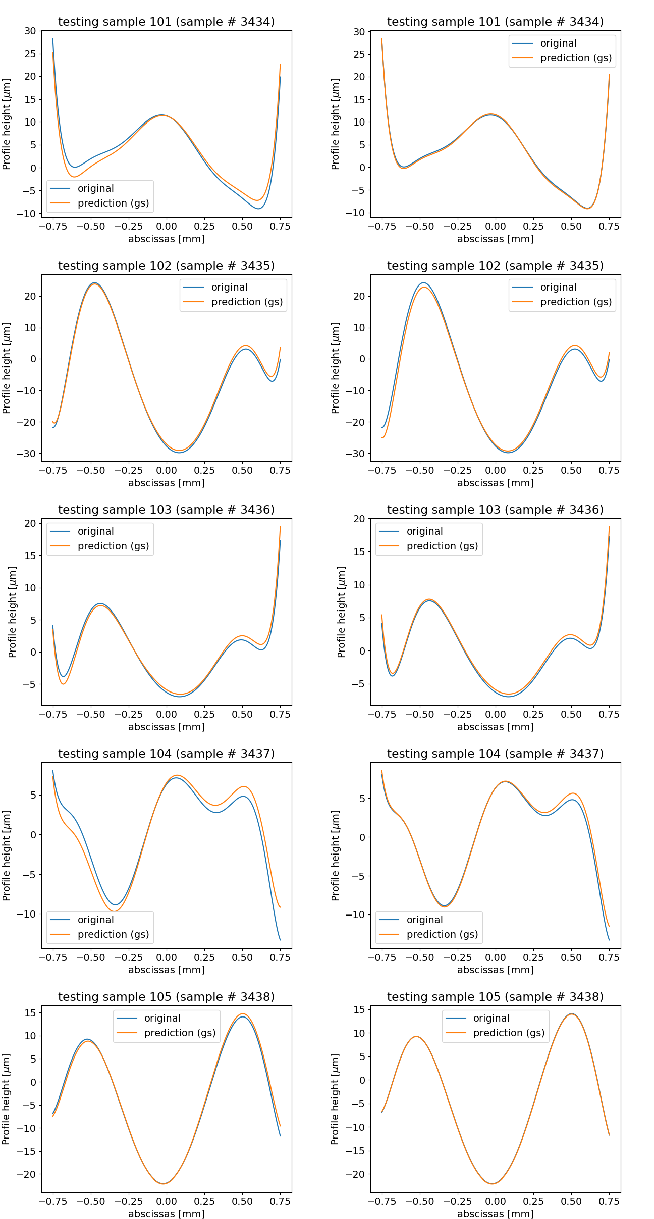
\includegraphics[width=0.75\textwidth]{figures/figure_multimode.pdf}
% 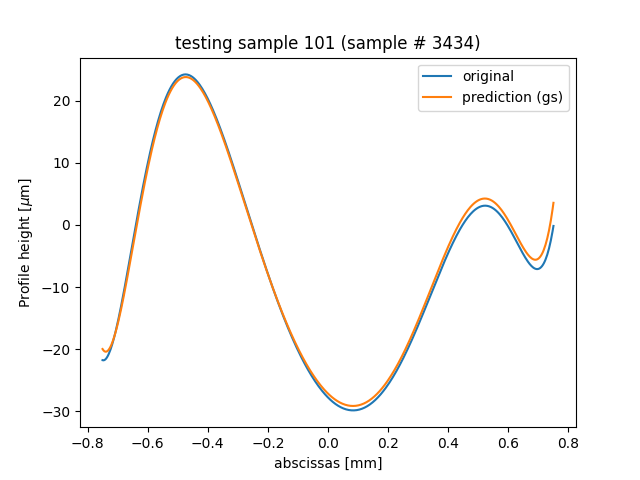
\includegraphics[width=0.45\textwidth]{figures/v20p101.png}
% 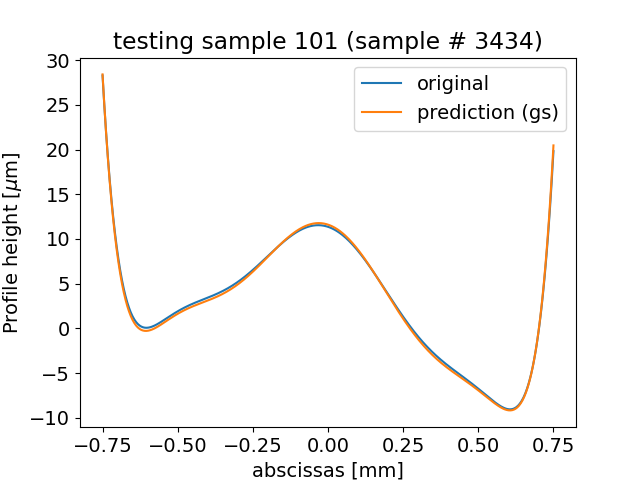
\includegraphics[width=0.45\textwidth]{figures/v23p101.png}

% 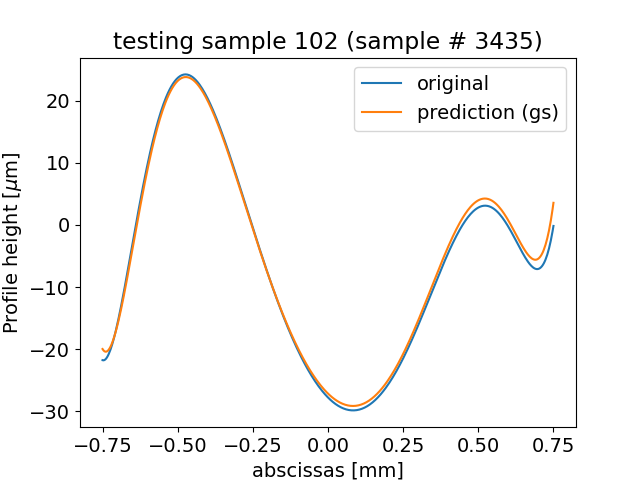
\includegraphics[width=0.45\textwidth]{figures/v20p102.png}
% 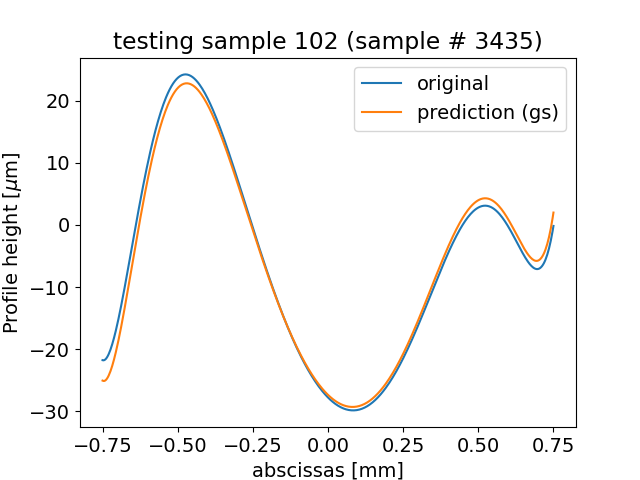
\includegraphics[width=0.45\textwidth]{figures/v23p102.png}

% 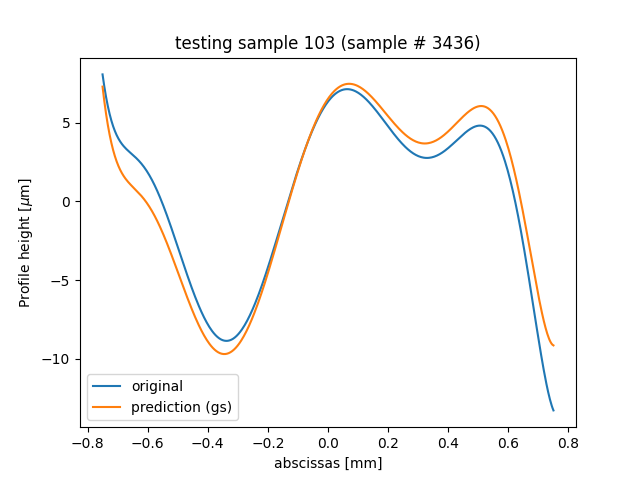
\includegraphics[width=0.45\textwidth]{figures/v20p103.png}
% 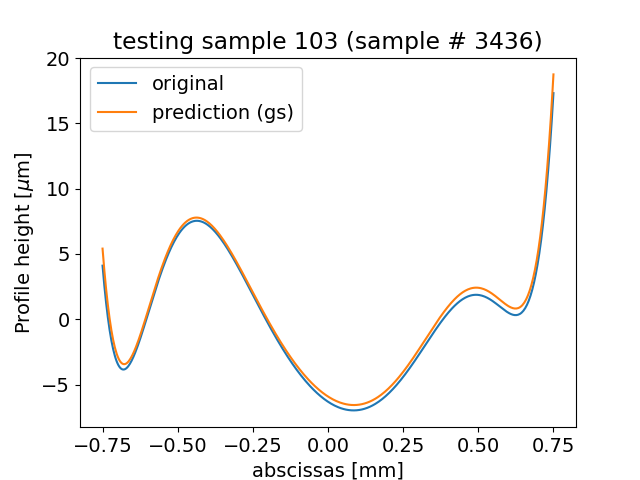
\includegraphics[width=0.45\textwidth]{figures/v23p103.png}

% 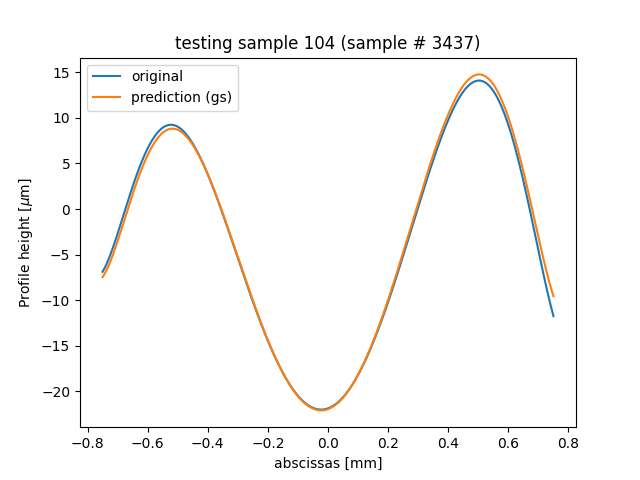
\includegraphics[width=0.45\textwidth]{figures/v20p104.png}
% 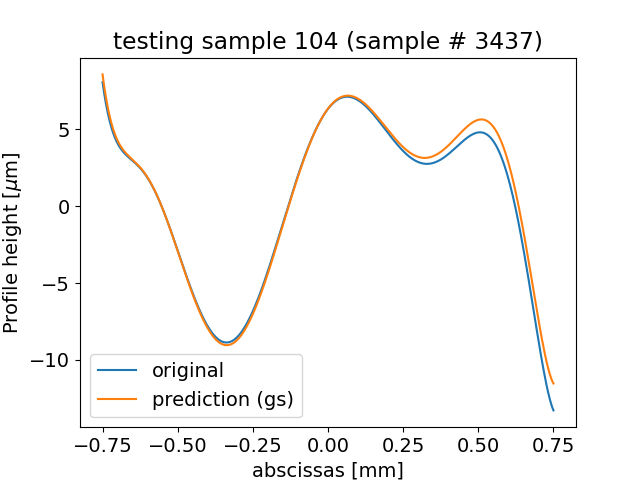
\includegraphics[width=0.45\textwidth]{figures/v23p104.png}

% 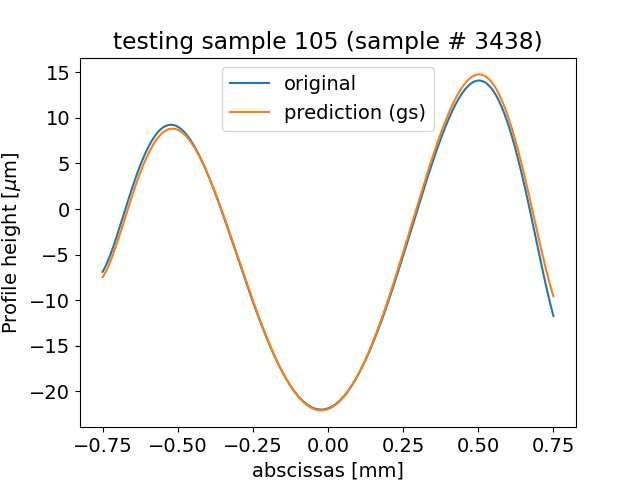
\includegraphics[width=0.45\textwidth]{figures/v20p105.png}
% 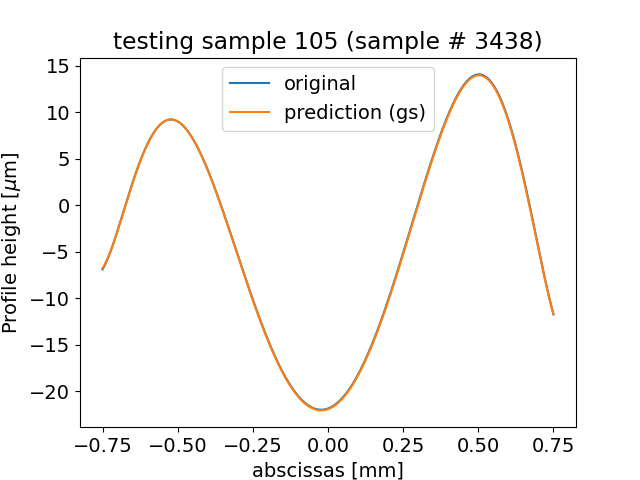
\includegraphics[width=0.45\textwidth]{figures/v23p105.png}
\caption{
Some original and fitted (predicted) profiles from samples in the test data. We used here multimode partial coherence.
a) (left column) 1500 epochs;
accuracy on test data 92.3\%. 
b) (right column) 24000 epochs;
accuracy on test data 96.7\%.
    }
\end{figure}


\subsection{Effect the abscissas interval used the errors}
The learning process for the CRL with 10 lenses is worse (see Fig.~\ref{fig:v12v13}c) than for the single lens (Fig.~\ref{fig:v12v13}b). This is related to the illuminated area. Indeed, the larger absorption of the 10 lenses makes that the illumination just after the CRL is smaller for the multi-lens CRL as compared to the single-lens CRL. Obviously, the CNN cannot predict the correct profile in a zone that is not illuminated, because the propagated intensity profiles have no changes if the error profile changes only in the dark side. To test this, we adjusted the abscissas interval of the generated random profiles to better match the illuminated area. As expected, we obtained better results (see Fig.\ref{fig:v26profiles}).

\begin{figure}\label{fig:v26profiles}
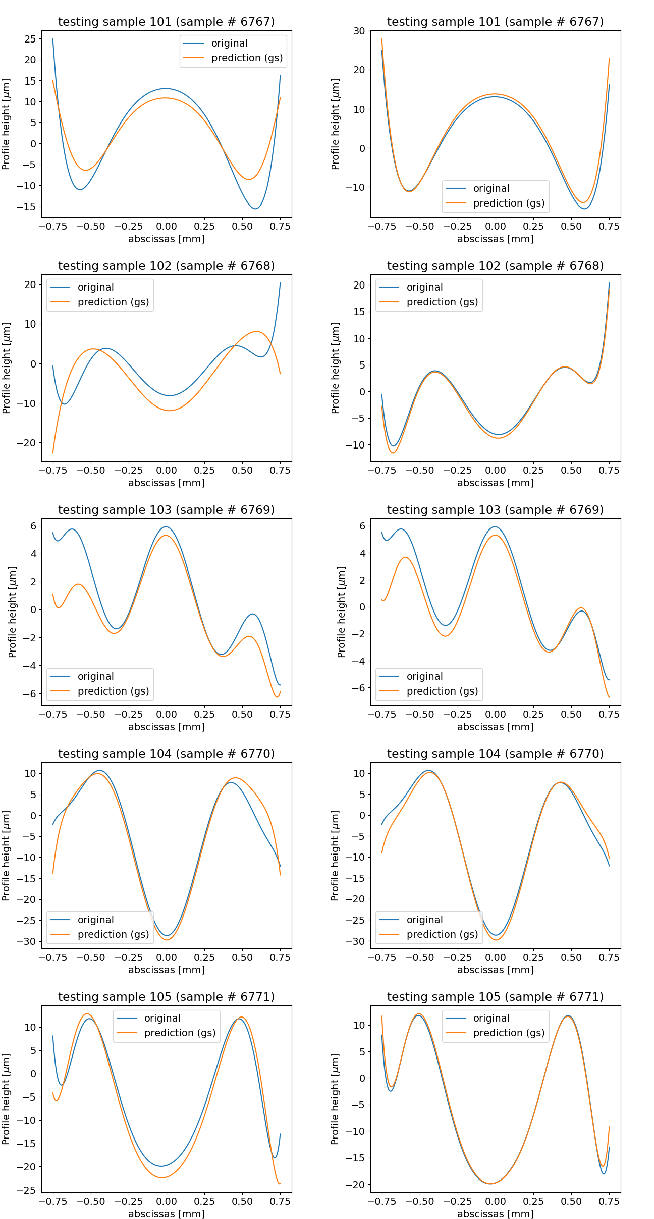
\includegraphics[width=0.75\textwidth]{figures/figure7.pdf}
% 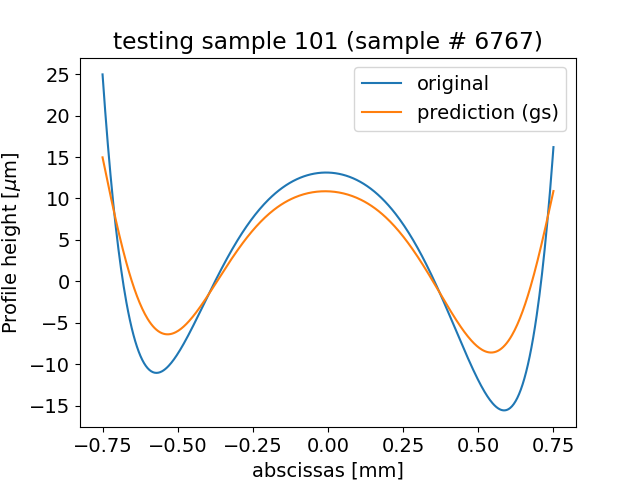
\includegraphics[width=0.45\textwidth]{figures/v25p101.png}
% 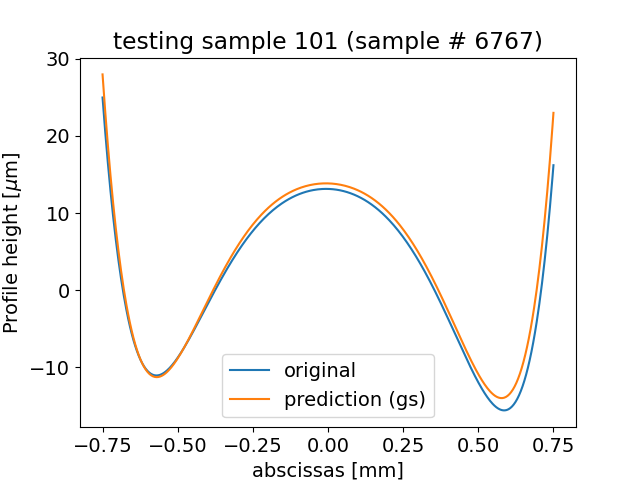
\includegraphics[width=0.45\textwidth]{figures/v26p101.png}

% 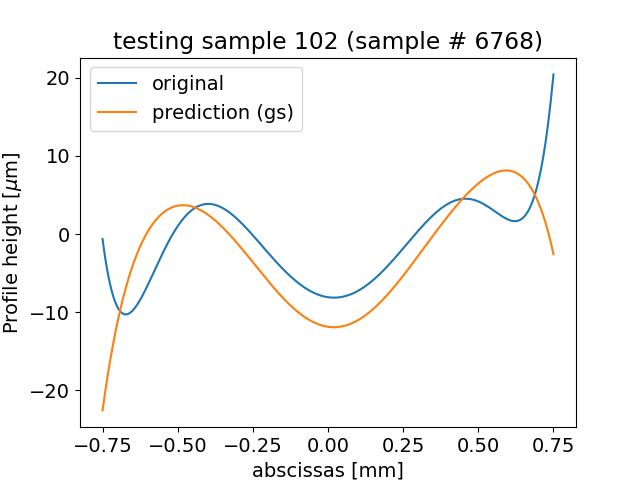
\includegraphics[width=0.45\textwidth]{figures/v25p102.png}
% 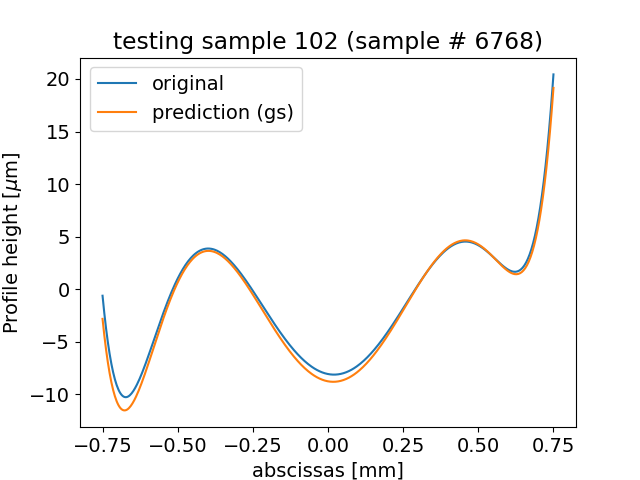
\includegraphics[width=0.45\textwidth]{figures/v26p102.png}

% \includegraphics[width=0.45\textwidth]{figures/v25p103.png}
% \includegraphics[width=0.45\textwidth]{figures/v26p103.png}

% \includegraphics[width=0.45\textwidth]{figures/v25p104.png}
% \includegraphics[width=0.45\textwidth]{figures/v26p104.png}

% \includegraphics[width=0.45\textwidth]{figures/v25p105.png}
% \includegraphics[width=0.45\textwidth]{figures/v26p105.png}
\caption{
Some original and fitted (predicted) profiles from samples in the test data for the multi-lens CRL case. a) (left column) error profiles defined over a window of \SI{1500}{\micro\meter};
accuracy on test data 72.6\%. 
b) (right column) error profiles defined over a window of \SI{800}{\micro\meter};
accuracy on test data 84.7\%.
    }
\end{figure}

\subsection{Zernike coefficients from full random recipe}
The algorithm used samples the coefficients for the different Zernike polynomials using a phenomenological model resulting from the analyses of experimental error profiles made in previous works. We tested this model against the full random model (all  coefficients are created using a random uniform distribution in [0,\SI{5}{\micro\meter}]). The algorithm based on the phenomenological recipe works better (0.726 accuracy) than a fully random generation of the coefficients from uniform distributions (0.562 accuracy). This is because in our model there is in some way coded the effect of the illumination profile on the CRL. This is true for the \SI{1500}{\micro\meter} window where, as discussed before, include non-illuminated areas. If we reduce the window, both algorithms produce similar results. 

\subsection{Effect of inaccuracies in error profiles on the propagated images.}
We have always measured the accuracy of the CNN by comparing the guessed error profile with the true error profile. Even when the accuracy is not excellent, for example in Fig. \ref{fig:v26profiles}a, the guessed profile usually separates from the true profile only at the edges. In these areas the transmitted intensity is low and therefore the effect of this discrepancy is small in the propagated intensity profiles. To illustrate this phenomenon, we compared the propagated wavefronts using the true error profile and the guessed error profile for the sample 103 in \ref{fig:v26profiles}. The results show a very similar intensity distributions (Fig. \ref{fig:figure8}).

\begin{figure}\label{fig:figure8}
\includegraphics[width=0.85\textwidth]{figures/figure8.png}

\caption{
Intensity distributions for the multi-lens CRL at the central plane of the propagation interval for the profile 103 in Fig.~\ref{fig:v26profiles}. The three distributions refer to the true sampled profile, the guessed profile when a window of $\SI{1500}{\micro\meter}$, and the guessed profile when a window of $\SI{800}{\micro\meter}$. We only observe  minimum differences in the intensity distributions.
    }
\end{figure}

\section{Conclusions}\label{sec:conclusions}

We have shown in this work that a CNN trained with synthetic data is able to retrieve the profile error in an x-ray lens giving as input a set of intensity distributions measured or calculates at different positions. The trained CNN is a robust model that works satisfactorily in many conditions. Many tuning parameters that can be changed in the CNN and also physical phenomena like the number of planes used or the effect of partial coherence have been analyzed and, although showing more or less sensitivity to the accuracy of the results, they always produce reasonably good results. This feasibility study opens the way to other more complete analyses. The next effort will consist in dealing with 2D wavefronts and images. This will certainly increase the amount of data and retard the learning process, but there is no reason for not getting similar good results. The usefulness of the CNN trained with synthetic data and being fed with  experimental images will be addressed in a future work.  


%-------------------------------------------------------------------------
%-------------------------------------------------------------------------

%-------------------------------------------------------------------------

% \ack{\textbf{Funding information}}
% This project has received funding from the European Union’s Horizon 2020 Research and Innovation Programme under grant agreements: N$^{\circ}$ 823852 (Photon and Neutron Open Science Cloud -- PaNOSC); N$^{\circ}$ 101007417 (NFFA-Europe Pilot Joint Activities -- NEP) and N$^{\circ}$ XXX

%-------------------------------------------------------------------------
% \ack{\textbf{Acknowledgements}}
%-------------------------------------------------------------------------

% To the people who provided the samples for being measured. To the scientists who provided the experimental data and access to their beamlines.


% -----------------------------------------------------------------
\ack{\textbf{Data availability}}
% -----------------------------------------------------------------

Data underlying the results presented in this paper are publicly available at (accessed: 12/01/2024):
\begin{center}
\small{\texttt{https://github.com/rafaelcelestre/mlcrl/}}
\end{center}

% -----------------------------------------------------------------

\referencelist{iucr}



\end{document}                    % DO NOT DELETE THIS LINE
%%%%%%%%%%%%%%%%%%%%%%%%%%%%%%%%%%%%%%%%%%%%%%%%%%%%%%%%%%%%%%%%%%%%%%%%%%%%%%
